\section{Basic Fluid Dynamics}
\thispagestyle{plain}

Fluids (gases or liquids\footnote{In gases, time between interactions is so much longer than
time of interactions that they can often be described by kinetic gas theory. At higher temperatures
there are more collsions and the gas is more viscous while in liquids at higher temperatures \textit{bonds are easier to break}
so the liquid is less viscous.}) react to tangential (aka shear) stress with flow, a deformation
rate depending on the viscosity, as opposed to solids which deform. Many systems from galaxies
to lab plasmas can - on the right scale - be successfully modelled as fluids.

\subsection{Basic notes on fluid description - the fluid from the view of a parcel - macroscopic fluid view}
Physical systems can be described on different level: from a wave function in quantum physics,
over a collection of point-like particles in classical physics to a \textbf{continuous fluid}.

\subsubsection{When is a fluid description valid?}
We want to describe the fluid in terms of macroscopic position and time dependent quantities like:
mass density $\rho$, temperature $T$, velocity $\vec{u} = \vec{v} + \vec{w}$ where $\vec{v} = \langle \vec{u} \rangle$
is the mean (bulk) velocity of the local fluid element and $\vec{w}$ is the random velocity defining the
temperature.
\subsubsubsection{Connection between temperature and random movement}
As of the equipartition theorem, each exitable degree of freedom adds $\frac{k_BT}{2}$ to the
internal energy, so
\begin{equation}
    \langle \frac{1}{2} m w_i^2 \rangle = \frac{1}{2} k_B T \quad \rightarrow \quad \langle ||\vec{w} ||^2 \rangle = \frac{3k_BT}{m}
\end{equation}

\subsubsubsection{Continuum Hypothesis}
Q: When does it make sense to describe a physical system by a continuous fluid? A: When we can construct
a volume small compared to the region of the fluid but big compared to the molecular free path. When
we consider a fluid in terms of \textbf{parcels} with constant mass and particle number
\begin{equation}
    \text{parcel mass } m_p = \int_{V} \rho dV, \quad \text{parcel volume } V, \quad \text{parcel density } \rho
\end{equation}
we postulate that every fluid quantity (bulk quantity of the parcel) tends to a limit as the size of the volume
approaches zero, before molecular fluctuation kicks in (\textbf{continuum hypothesis}), see figure \ref{fig:continuum_hypothesis}.

\begin{figure}[!htb]
 \centering
 \includesvg[width=0.8\textwidth]{figures/continuum.svg}\hfill
 \caption{Continuum hypothesis; REV = representative elementary volume}
 \label{fig:continuum_hypothesis}
\end{figure}

\begin{mdframed}[style = padded]
    A fluid description is thus justified if
    \begin{equation}
        \text{Knudsen number } Kn = \frac{\text{mean free path of particles } \lambda_{mfp}}{\text{characteristic system length } L} \ll 1
    \end{equation}
\end{mdframed}

\subsubsection{Example: the plasma in the intercluster medium can be considered a fluid\skipthis}
\subsubsubsection{Mean free path in a model of colliding spheres}
\label{ssssec:mean_free_path}
Consider a particle has a collisional cross-section of $\sigma$ (in $\m^2$) and moves with root mean square velocity
$\bar{v}$ in a medium with number density $n$ (in $\m^{-3}$). Note that the mean relative velocity
between particles is larger than the mean velocity per particle
\begin{equation}
    \langle v_{rel}^2 \rangle = \langle (v-v')^2 \rangle = \langle v^2 \rangle - \explain{2 \langle vv' \rangle}{$=0$, as uncorrelated} + \langle v'^2 \rangle = 2 \langle v'^2 \rangle = 2 \bar{v}^2 \quad \rightarrow \quad v_{rel} = \sqrt{2} \bar{v}
\end{equation}
A particle thus in a time $\tau$ probes the volume $V = \sigma v_{rel} \tau$, so interacts with $N = nV$ particles. We
are interested in the time till one interaction so the case $N = 1$, so $\tau = \frac{1}{n v_{rel} \sigma}$. The path
the particle itself has moved during that time is
\begin{equation}
    \lambda_{mfp} = \tau \bar{v} = \frac{1}{\sqrt{2} n \sigma}
\end{equation}
\note{The electrons though are much more mobile than the protons ($\frac{m_e}{m_p} \approx \frac{1}{1836}, m_e \approx 10^{-30}$ kg) so for electron-ion collisions the simpler $\lambda_{mfp} = \frac{1}{n \sigma}$ (assuming stationary nuclei) is probably better.}
\subsubsubsection{Collisional cross-section of an electron in a plasma and first approximation of $\lambda_{mfp}$}
We approximate $\sigma = \pi r_{eff,e}^2$. We can approximate this radius by the distance where the electrostatic potential
(in the electron-ion or electron-electron interaction) is only as relevant as the thermal energy, so ($Z$ for the nucleic charge,
relevant for the ion-electron interaction)
\begin{equation}
    \frac{Ze^2}{r_{eff,e}} \sim m_e w_e^2 \sim k_B T_e
\end{equation}
We can therefore approximate an electron mean free path
\begin{equation}
    \begin{aligned}
        \lambda_{mfp,e} &\simeq \frac{1}{n\sigma} \sim \frac{1}{n\pi r_{eff,e}^2} \sim \frac{1}{\pi n} \left( \frac{k_B T_e}{Ze^2} \right) \\
                        &\sim 1.5 \times 10^{22} \left( \frac{n}{10^{-3} \cm^{-3}} \right)^{-1} \left( \frac{k_B T_e}{1 \keV} \right) \cm
    \end{aligned}
\end{equation}
where we assumed $Z = 1$.
\note{Most \textit{collisions} in (strongly ionized) plasmas are Coulomb interactions with very small deflections (so collision parameters mostly larger than $r_{eff,e}$). Therefore, we define the collision rate and collisional cross-section based on a total deflection of $\frac{\pi}{2}$.}

\subsubsubsection{A better approximation to the mean free path in an ionized plasma}
More careful considerations take into account the smaller deflections. The integral over $\frac{1}{b}$
(impact parameter $b$) yields the
Coulomb logarithm
\begin{equation}
    \log \Lambda = \log \frac{b_{max}}{b_{min}}
\end{equation}
where for $b_{max}$ we take the Debye length
\begin{equation}
    \lambda_{D\xi} = \left( \frac{\epsilon_0 k_B T_\xi}{n_\xi e^2} \right) ^ \frac{1}{2}, \quad \xi = \text{ion, electron}, \quad \text{in plasma } n_i \approx n_e
\end{equation}
(where the potential of a \textit{Überschussladung} drops to $\frac{1}{e} \phi_0$ ($e$ here Euler's number))
and for $b_{min}$ e.g. $\pi r_{eff,e}$. One finally gets
\begin{equation}
    \lambda_{mfp,e} = \frac{\bar{v_e}}{\nu_{ei}} \approx 64 \pi \lambda_D \frac{\Lambda}{\log \Lambda} \propto \frac{T_e^2}{n_e} \gg \lambda_D
\end{equation}
with $\nu_{ei}$ being the electron-ion collision rate. Examples of mean free paths are given in table \ref{tab:mean_free_path}.

\begin{table}[!htb]
    \centering
    \begin{tabular}{|p{0.2\textwidth}|p{0.2\textwidth}|p{0.2\textwidth}|p{0.2\textwidth}|}
        \hline
        \textcolor{blue1}{Plasma} & Solar Wind ($n \sim 1 \cm^{-3}, T = \text{some } \eV$) & Ionosphere & Gas molecule in air under standard conditions \\
        \hline
        \textcolor{blue1}{mean free path $\lambda_{mfp}$} & $1$ AU & $1 \km$ & $68$ nm \\
        \hline
    \end{tabular}
    \caption{Mean free paths}
    \label{tab:mean_free_path}
\end{table}
The plasma in the intercluster medium can be considered a fluid. The solar wind can hardly be considered a fluid
on a reasonable scale.

\subsubsection{Fluid description based on fluid parcels}
The modes of motion in a fluid are
\begin{itemize}
    \item motion of macroscopic fluid parcels
    \item random walk between fluid parcels (diffusion, very slow)
\end{itemize}
The most important fluid equation, the \textbf{Navier Stokes equation} \textit{falls out of the} Boltzmann equation
but can also be \textit{understood} as an equation of movement for a fluid parcel.
\begin{itemize}
    \item mass conservation $\Longleftrightarrow$ continuity equation
    \item mass conservation + momentum conservation $\Longleftrightarrow$ Navier Stokes equation
\end{itemize}

\subsubsubsection{Eulerian and Lagrangian fluid dynamics}
Lagrangian and Eulerian view are presented in table \ref{tab:lagrangian_eulerian}.

\begin{table}[!htb]
    \centering
    \begin{tabular}{|p{0.45\textwidth}|p{0.45\textwidth}|}
        \hline
        \textcolor{blue1}{Lagrangian description} & \textcolor{blue1}{Eulerian description} \\
        \hline
        Coordinate system comoves with the fluid element (we sit on the fluid parcel) & Coordinate system is fixed in space \\
        \hline
        The temporal evolution of fluid quantities is described along the trajectory of the movement of a fluid parcel & The temporal evolution of fluid quantities is described at a fixed locations over accounting volumes \\
        \hline
        e.g. measurement on a weather balloon following the wind flow & e.g. measurement by ground stations \\
        \hline
    \end{tabular}
    \caption{Lagrangian and Eulerian fluid dynamics}
    \label{tab:lagrangian_eulerian}
\end{table}

The rate of change of a fluid variable (like temperature) along the
motion of a fluid parcel along the velocity field $\vec{v}$ (expressed in terms of Eulerian derivatives) 
is the \textbf{material derivative}. Let $\Psi_L(t)$ describe
the evolution of a fluid quantity along the parcel motion (Lagrangian) and $\Psi_E(\vec{x},t)$ the evolution of a fluid
quantity at a fixed location (Eulerian). Then the material derivative is
\begin{equation}
    D_t \Psi_L = \frac{D\Psi_L}{Dt} = \partial_t \Psi_L =  \explain{\partial_t \Psi_E}{local change} + \explain{\vec{v} \cdot \vec{\nabla}_\vec{x} \Psi_E}{convective change} = D_t \Psi_E
\end{equation}
(derive $\Psi(\vec{x}(t),t)$ with respect to time and use the chain rule).

Generally
\begin{equation}
    D_t = \partial_t + \vec{v} \cdot \vec{\nabla}
\end{equation}

We sometimes speak of \textbf{advection} if a scalar quantity is transported by the flow, and of \textbf{convection} if a vector quantity is transported by the flow
(but they are often also used synonymously and with different meanings in different contexts).

\subsubsubsection{Continuity equation}
As of mass conservation, the change of mass $m_V$ in a volume $V$ can only be due to flux $\vec{j} = \rho \vec{v}$ through the surface $\partial V$.
\begin{equation}
    \partial_t m_V = \partial_t \int_V \rho dV = - \int_{\partial V} \vec{j} \cdot d\vec{A} \explain{=}{Gauss} - \int_V \vec{\nabla} \cdot \vec{j} dV \quad \rightarrow \quad \boxed{\partial_t \rho + \vec{\nabla} \cdot (\rho \vec{v}) = 0}
\end{equation}
which is the continuity equation.

\subsubsubsection{Incompressible fluids}
An incompressible fluid is one, where the density of a fluid parcel never changes with time $\frac{d\rho}{dt} = 0$ (there can still be gradients in the density). From the material derivative form of the continuity equation
\begin{equation}
    0 = \frac{d\rho}{dt} = \partial_t \rho + \vec{v} \cdot \vec{\nabla} \rho \explain{=}{cont. eq.}  \quad \rightarrow \quad \boxed{\vec{\nabla} \cdot \vec{v} = 0}
\end{equation}
For $\vec{\nabla}\cdot \vec{v} < 0$ we have a sink, for $\vec{\nabla}\cdot \vec{v} > 0$ a source.
The divergence of the velocity field of incompressible fluids vanishes (divergence free flow) (e. g. rotational flow)
Note in a 3D flow horizontal convergence can be balanced by vertical divergence.
\paragraph{Interpretation of $\vec{\nabla}\cdot \vec{v} = 0$} A divergence free flow does not mean that the velocity does not change over space as one can easily see from flow along a narrowing tube.
Consider a tube with flow tangential to it.
\begin{equation}
    \begin{gathered}
    \vec{\nabla} \cdot \vec{v}=0 \xrightarrow{\text { integrate over tube }} 0=\int_V \vec{\nabla} \cdot \vec{v} d V \underset{\text { Gauss }}{=} \int_{\partial V} \vec{v} d \vec{A} \\
    \xrightarrow[\text { only opposing flux trough } A_1 \text { and } A_2]{} v_1 A_1-v_2 A_2=0 \\
    \rightarrow v_1 A_1=v_2 A_2
    \end{gathered}
\end{equation}

\subsubsubsection{Equation of motion of a fluid parcel, general path towards Navier-Stokes}
Consider a fluid parcel with constant mass $m$. The equation of motion is
\begin{equation}
    \vec{F} = \frac{d\vec{p}}{dt} = m \frac{d\vec{V}}{dt} = \rho V \frac{d\vec{v}}{dt}, \quad \vec{a} = \frac{\vec{F}}{\rho V} = \frac{\vec{f}}{\rho} = \frac{d\vec{v}}{dt}
\end{equation}
Using the material derivative, we can write
\begin{equation}
    \frac{d\vec{v}}{dt} = \partial_t \vec{v} + \underbrace{\vec{v} \cdot \vec{\nabla} \vec{v}}_{\parbox{8em}{\footnotesize non-linear advective term $\rightarrow$ chaotic behavior}} = \vec{a} = \frac{\vec{f}}{\rho}
\end{equation}
where one can find (leading to a simplified \textbf{Navier Stokes equation})
\begin{equation}
    \vec{f} = \underbrace{\vec{f}_{g}}_{\parbox{4em}{gravi. force}} + \underbrace{\vec{f}_{p}}_{\parbox{4em}{pressure force}} + \underbrace{\vec{f}_{f}}_{\parbox{4em}{friction force}} = \rho \vec{g} - \vec{\nabla} p + \rho \nu \vec{\nabla}^2 \vec{v}
\end{equation}
where the viscous friction $\vec{f}_v$ (viscosity $\nu$) is an approximation for an incompressible isotropic Newtonian fluid.
While pressure is a force per area, only when there are different pressures acting on the sides of a fluid parcel (a gradient), there is net movement.
The friction term can be understood as diffusion of momentum when there is a velocity gradient (which only leads to a local change when
when $\vec{\nabla}^2 \vec{v} \neq 0$, otherwise there is the same momentum diffusion in and out of the parcel).

\subsection{Basic Gas Dynamics}
\greenbox{\textbf{Aim:} Our aim is to derive equations for the evolution of variables of the fluid, like density, velocity and temperature. For instance
how do perturbation (e.g. by a jet) propagate through the fluid?}
\subsubsection{Distribution function and Boltzmann equation}
\idea{Let us derive the fluid equations based on the Boltzmann equation for the distribution function.}
The distribution function $f(\vec{x}, \vec{u},t)$ is defined so that
\begin{equation}
    f(\vec{x},\vec{u},t) d^3xd^3u
\end{equation}
is (depending on the normalization) the probability of finding a particle in the
phase space volume $d^3xd^3u$ around $(\vec{x},\vec{u})$ at time $t$ or the expected
number or particles therein, so in total
\begin{equation}
    N = \int \int f(\vec{x},\vec{u},t) d^3xd^3u, \quad \text{total number of particles } N
\end{equation}
\begin{mdframed}[style = padded]
    Phase space conservation (Liouville theorem) (particles are neither created nor destroyed) is captured in the Boltzmann equation
    \begin{equation}
        \frac{d}{dt} f(\vec{x},\vec{u},t) = \partial_t f + \vec{\dot{x}} \vec{\nabla}_\vec{x} f + \vec{\dot{u}} \vec{\nabla}_\vec{u} f = \left. \frac{df}{dt} \right|_c, \quad \text{with } \vec{\dot{x}} = \vec{u}, \vec{\dot{u}} = \vec{g}
    \end{equation}  
    where $\left. \frac{df}{dt} \right|_c$ is the change in $f$ due to \textit{collisions}. 
\end{mdframed}
\note{One can understand this in the sense of dicontinupus motion (instantaneous velocity changes) kicking a particle out of a phase space volume.
More aligned with our previous derivation, we can see this as a simplification of the correlation term between forces and accelerations (also capturing the
particle interaction) (see subsection \ref{subsec:particle_to_boltzmann}).}
In the case of a sufficiently large collision term $\left. \frac{df}{dt} \right|_c$ (in the fluid limit $\lambda_mfp\ll L$) $f(\vec{u})$
becomes Mawellian. Near the sun for instance Coulomb collisions are incapable of isotropizing the velocity distribution of the 
ions in the solar wind (cigar shape).

\subsubsection{Retrieving information from the Boltzmann equation}
By taking the \textcolor{blue1}{moments of the distribution function over velocity space}
\begin{equation}
    M_n(\vec{x},t) = \int \vec{v}^n f(\vec{x},\vec{u},t) d^3u
\end{equation}
we find out on the quantities of interest in space as
\begin{itemize}
    \item \textcolor{blue1}{density} (0th moment)
    \begin{equation}
        \begin{gathered}
            n = \int f(\vec{x},\vec{u},t) d^3u, \quad \rho = nm, \quad \text{particle mass } m \\
            \rightarrow \text{mass weighted average } \langle q \rangle (\vec{x},t) = \frac{1}{\rho(\vec{x})} \int q(\vec{x},\vec{u},t) f(\vec{x},\vec{u},t) d^3u 
        \end{gathered}
    \end{equation}
    \item \textcolor{blue1}{mean velocity} (1st moment)
    \item \textcolor{blue1}{pressure tensor} as of the fluctuations of the velocity around the mean ($\rightarrow$ temperature in case of a Maxwell distribution) (2nd moment)
    \item \textcolor{blue1}{heat tensor} (3rd moment)
\end{itemize}
The development of those quantities in time is given by the \textcolor{blue1}{balance (/conservation) equations obtained from
taking the appropriate moments of the Boltzmmann equation (mass, momentum and energy are conserved)}.
\begin{equation}
    \text{form of balance equations: } \partial_t\text{conserved quantity} + \vec{\nabla}\text{corrsp. flux} = \text{source term} 
\end{equation}

\subsubsection{Mass conservation | continuity equation (0th moment)}
By following the steps
\begin{itemize}
    \item multiply the Boltzmann equation by $m$ and integrate over $d^3u$
    \item using Gauss divergence theorem and assuming $f \rightarrow 0$ for $u \rightarrow \infty$
    \item local mass conservation $\int m \left. \frac{df}{dt} \right|_c d^3u = 0$ (collisions only shift discontinuously on velocity space)
\end{itemize}
one follows the mass continuity equation
\begin{mdframed}[style = padded]
\begin{equation}
    \partial_t\rho + \vec{\nabla} \cdot (\rho \cdot \vec{v}) = 0, \quad \vec{u} = \vec{v} + \vec{w}, \quad \vec{v} = \langle \vec{u} \rangle
\end{equation}
\end{mdframed}
By taking the volume integral ($d^3x$) we find $\frac{dm}{dt} = 0$, i.e. mass conservation.
\subsubsubsection{Derivation of the continuity equation\skipthis}
From
\begin{equation}
    \explain{\int m \partial_t f d^3u}{$\partial_t\rho(\vec{x},t)$} + \underbrace{\vec{\nabla}_\vec{x} \int m \vec{u} f d^3u}_{\parbox{6em}{\footnotesize using $r$,$u$ indep.; $=\vec{\nabla}_\vec{x} (\rho \vec{v})$}} + \explain{\int m \vec{\nabla}_\vec{u} (\vec{g} f) d^3 u}{assume acc. $\vec{g}$ indep. $\vec{u}$} = \explain{\int m \left. \frac{df}{dt} \right|_c d^3u}{$=0$ (local particle conserv.)}
\end{equation}
where the third term also vanishes (apply Gauss, assume $f \rightarrow 0$ (e.g. Maxwellian $\exp(-u^2)$) for $u \rightarrow \infty$), we get the result from above.

\subsubsection{Momentum conservation | Navier Stokes equation (1st moment)}
By following the steps
\begin{itemize}
    \item multiply Boltzmann equation with momentum ($m\vec{u}$) and integrate over $d^3u$
    \item using that collisions conserve momentum
    \item using the continuity equation
\end{itemize}
\begin{mdframed}[style = padded]
one obtains the Navier-Stokes equation
\begin{equation}
    \partial_t (\rho \vec{v}) + \vec{\nabla} \cdot (\rho \vec{v}\vec{v}^T + P\mat{1} - \mat{\Pi}) = \rho \vec{g}
\end{equation}
which using the continuity equation becomes
\begin{equation}
    \partial_t \vec{v} + (\vec{v} \cdot \vec{\nabla}) \vec{v} = \vec{g} - \frac{1}{\rho} \vec{\nabla}P + \frac{1}{\rho} \vec{\nabla} \cdot \mat{\Pi}
\end{equation}
with
\begin{equation}
    \begin{gathered}
        \text{(isotropic) pressure } P = \frac{1}{3} \rho \langle ||\vec{w}||^2 \rangle \\
        \text{anisotropic viscous stress tensor } \Pi_{ij} = P\delta_{ij} - p \langle w_iw_j \rangle \text{ (symmetric and traceless)} \\
        \text{acceleration }\vec{g} \text{ from external sources }
    \end{gathered}
\end{equation}
Viscosity opposes shearing motion and interprenetation (diffusion of momentum on shear).
\end{mdframed}
Taking the volume integral over the Navier-Stokes equation and applying Gauss theorem, we see that in the absence
of an external force ($\vec{g} = 0$), the momentum is conserved.
\subsubsubsection{Notes on the derivation of the Navier-Stokes equation}
Take a look at the terms in
\begin{equation}
     \partial_t \int m \vec{u} f d^3u + \vec{\nabla}_\vec{x} \int m \vec{u} \vec{u}^T f d^3u + \int m \vec{g} \vec{u}^T \vec{\nabla}_\vec{u} f du^3 = \int m \vec{u} \left. \frac{\partial f}{\partial t} \right|_c d^3u 
\end{equation}
\begin{itemize}
    \item first term: $\partial_t \int m \vec{u} f d^3u = \partial_t (\rho \vec{v})$ by definition of $\vec{v}$
    \item second term: $\vec{\nabla}_\vec{x} \int m \vec{u} \vec{u}^T f d^3u = \vec{\nabla}_\vec{x} \left(\rho \langle \vec{u} \vec{u}^T \rangle\right)$ using $\vec{u} = \vec{v} + \vec{w}$
    this becomes $\vec{\nabla}_\vec{x} \left(\rho \vec{v} \vec{v}^T \right) + \mathcolor{red1}{2 \vec{\nabla}_\vec{x} \left(\rho \vec{v} \langle \vec{w} \rangle^T \right)} + \vec{\nabla}_\vec{x} \left(\rho \langle \vec{w} \vec{w}^T \rangle\right) = \vec{\nabla}_\vec{x} \left(\rho \vec{v} \vec{v}^T \right) + \vec{\nabla}_\vec{x} \left(\rho \langle \vec{w} \vec{w}^T \rangle\right)$ as $\langle \vec{w} \rangle = \vec{0}$.
    \item third term: assuming $\vec{g}$ does not depend on $\vec{u}$, $\vec{g} \int m \vec{u}^T \vec{\nabla}_\vec{u} f du^3 = -\rho \vec{g}$ as by the chain rule $\vec{u}^T \vec{\nabla}_\vec{u} f = \vec{\nabla}_\vec{u} (\vec{u}^T f) - f \vec{\nabla}_\vec{u} \vec{u}^T$ where the integral over the first term vanishes by the same reasoning as before
    \item the right-hand side vanishes, because collisions conserve momentum
\end{itemize}
Finally, $\left(\rho \langle \vec{w} \vec{w}^T \rangle\right)$ (so the correlation matrix of the random fluctuations (?)) is split into an isotropic contribution from pressure $P$ and an
anisotropic viscous stress tensor $\mat{\Pi}$. The continuity equation can be used to get (first apply chain rule) $\partial_t (\rho \vec{v}) + \vec{\nabla}_\vec{x} \left(\rho \vec{v} \vec{v}^T \right) = \rho \left( \partial_t \vec{v} + (\vec{v}\cdot \nabla)\vec{v} \right)$

\subsubsubsection{Interpretation and viscous stress tensor for a Newtonian fluid}
Our result
\begin{equation}
    \frac{d\vec{v}}{dt} = \partial_t \vec{v} + (\vec{v} \cdot \vec{\nabla}) \vec{v} = \vec{g} - \frac{1}{\rho} \vec{\nabla}P + \frac{1}{\rho} \vec{\nabla} \cdot \mat{\Pi}
\end{equation}
already looks similar to our intuitive result. We have
\begin{itemize}
    \item some acceleration from external forces $\vec{g}$ (e.g. gravity)
    \item pressure force, where on the pressure we now also have a microscopic unterstanding $P = \frac{1}{3} \rho \langle ||\vec{w}||^2 \rangle$
    \item some viscous force as described by $\frac{1}{\rho} \vec{\nabla} \cdot \mat{\Pi}$
\end{itemize}

\greenbox{\textbf{Intuition for viscosity and momentum diffusion:} Viscosity is an every-day phenomenon - but how can we understand it miscroscopically?
Consider a fluid with bulk velocity $\vec{v}$ only in $x$-direction. Now imagine $v_x$ increases with $z$ (maybe because im pulling a plate on
top of my container). The molecules constantly bump into each other, and it is much more probabable that a particle from higher up $z$ will give $x$-
momentum to one from lower down in a collision than vice versa. Therefore $x$-momentum diffuses down. However if the $x$-velocity increases linearly
with $z$, $v_x(z)$ will not change, as there is as much momentum transport in as out of a given slice along $x$ at some height $z$. Therefore the simplest
diffusion equation for momentum is $\rho \partial_t v_x(z) = \nu \rho \partial_z^2 v_x$ (for a positive curvature more momentum diffuses down from the top
then goes out of the bottom). Speaking in terms of the fluctuations $\vec{w}$ from the bulk velocity $\vec{v}$, in the above scenario we expect particles
with high \textit{random} downward velocity $-w_z$ to be faster than their surrounding (high $w_x$), so we expect $- \langle w_z w_x \rangle > 0$.}

With the above intuition, it should make sense that
\begin{equation}
    \Pi_{ij} = P\delta_{ij} - p \langle w_iw_j \rangle
\end{equation}
and that we might make the ansatz of $\Pi_{ij}$ being linear in $\frac{\partial v_i}{\partial x_j}$
\begin{equation}
    \begin{aligned}
        \Pi_{ij} &= \eta D_{ij} + \xi \delta_{ij} (\vec{\nabla}\cdot \vec{v}) \\
        D_{ij} &= \frac{\partial v_i}{\partial x_j} + \frac{\partial v_j}{\partial x_i} - \frac{2}{3} \delta_{ij} (\vec{\nabla} \cdot \vec{v})
    \end{aligned}
\end{equation}
with $D_{ij}$ being the deformation tensor that vanishes for uniform expansion or contraction, $\eta$ and $\xi$ are the 
coefficients of shear and bulk viscosity respectively, with units $g \cm^{-1} \s^{-1}$.
\begin{itemize}
    \item $\eta D_{ij}$ represents the resistance to shearing motion
    \item $\xi \delta_{ij} \left( \vec{\nabla} \cdot \vec{v} \right)$ represents the resistance in volume, remember that for $\vec{\nabla} \cdot \vec{v} = 0$ we have an incompressible fluid
\end{itemize}

\subsubsection{Energy conservation (2nd moment)}
By the following steps
\begin{itemize}
    \item multiply the Boltzmann equation by $m\vec{u}^2$ and integrate over $d^3u$
    \item use that collisions conserve energy
    \item use the continuity equation
\end{itemize}
one follows
\begin{mdframed}[style = padded]
    \begin{equation}
        \begin{gathered}
            \rho \frac{de_{th}}{dt} \equiv \partial_t (\rho e_{th}) + \vec{\nabla} \cdot (\rho e_{th}\cdot \vec{v}) = -P \vec{\nabla}\cdot \vec{v} + \Psi - \vec{\nabla} \cdot \vec{Q} \\
            \text{specific internal energy } e_{th} \equiv \frac{1}{2} \langle ||\vec{w}||^2 \rangle \\
            \text{viscous dissipation rate (bulkmotion } \rightarrow \text{ internal energy) } \Psi \equiv \sum_{i,j=1}^{N} \Pi_{ij} \frac{\partial v_i}{\partial x_j} \\
            \text{conductive heat flux } \vec{Q} = \frac{1}{2} \rho \langle \vec{w} ||\vec{w}||^2 \rangle
        \end{gathered}
    \end{equation}
\end{mdframed}
\subsubsubsection{Notes on the conductive heat flux}
There is only conductive heat flux $\vec{Q}$ is $\vec{w}$ is asymmetric around the bulk motion (hotter (\textit{faster} in the sense of $||\vec{w}||$) particles drift relative to cold ones).
The conductive flux is in most cases produced by a temperature gradient
\begin{equation}
    \begin{gathered}
        \vec{Q} = -\xi \vec{\nabla} T, \quad \text{with } \chi \simeq 6 \times 10^{-7} T^{\frac{5}{2}} \text{erg} \s^{-1} \cm^{-1} \K^{-1} \\
        \text{proper diffusion coefficient } \kappa = \frac{\chi T}{P} \text{ in } \cm^2 \s^{-1}
    \end{gathered}
\end{equation}

(by collisions and random movement, wiggling spreads, stochastically along the gradient of $T$). As always, there is only change in a volume
if there is different in- and outflux, so if $\vec{\nabla} \cdot \vec{Q} \ne 0$.

\subsubsubsection{Evolution equation for the total specific energy $e = e_{th} + \vec{v}^2 / 2$}
We are interested in
\begin{equation}
    \frac{de}{dt} = \frac{de_{th}}{dt} + \frac{d}{dt} \left( \frac{1}{2} \vec{v}^2 \right)
\end{equation}
where we already know $\frac{de_{th}}{dt}$. So let us consider
\begin{equation}
    \begin{aligned}
    \partial_t \left( \frac{\rho \vec{v}^2}{2} \right) &= \frac{\vec{v}^2}{2} \mathcolor{blue1}{\partial_t \rho} + \rho \vec{v} \mathcolor{green1}{\partial_t \vec{v}} \\
    &= \frac{\vec{v}^2}{2} \mathcolor{blue1}{\left(-\vec{\nabla} (\rho \vec{v})\right)} + \rho \vec{v} \mathcolor{green1}{\left(-(\vec{v} \cdot \vec{\nabla}) \vec{v} + \vec{g} - \frac{1}{\rho} \vec{\nabla}P + \frac{1}{\rho} \vec{\nabla} \cdot \mat{\Pi}\right)} \\
    \end{aligned}
\end{equation}
where we used the \textcolor{blue1}{continuity equation} and \textcolor{green1}{Navier-Stokes equation}. Based on
\begin{equation}
    (\vec{v} \cdot \vec{\nabla}) \vec{v} \equiv \frac{1}{2} \vec{\nabla} \vec{v}^2, \quad \rho \vec{v} \frac{1}{2} \vec{\nabla} \vec{v}^2 + \frac{\vec{v}^2}{2} \vec{\nabla} \rho \vec{v} = \vec{\nabla} \cdot \left( \frac{1}{2} \rho \vec{v}^2 \vec{v} \right)
\end{equation}
this becomes
\begin{equation}
    \frac{d}{dt} \left( \frac{\rho \vec{v}^2}{2} \right) = \partial_t \left( \frac{\rho \vec{v}^2}{2} \right) + \vec{v} \cdot \left( \frac{1}{2} \rho \vec{v}^2 \vec{v} \right) = \rho \vec{v} \cdot \vec{g} - \vec{v} \cdot \vec{\nabla} P + \vec{v} \cdot \left( \vec{\nabla} \cdot \mat{\Pi} \right)
\end{equation}
\begin{mdframed}[style = padded]
so we finally get the evolution equation for the total specific energy $e = e_{th} + \vec{v}^2 / 2$
\begin{equation}
    \partial_t (\rho e) + \vec{\nabla} \cdot \left[(\rho e + P)\vec{v} - \mat{\Pi} \cdot \vec{v} + \vec{Q} \right] = \rho \vec{v} \cdot \vec{g}
\end{equation}
where taking the volume integral and applying Gauss theorem shows energy conservation if $\vec{g} =\vec{0}$.
\end{mdframed}

\subsubsection{Entropy conservation}
\note{Heat conduction and viscous friction change the entropy and entropy is conserved is those processses are absent.}
From the first law of thermodynamics in its specific form (specific volume $\tilde{V} = 1/\rho$)
\begin{equation}
    de_{th} = dw + dq = -P d\tilde{V} + Tds = \frac{P}{\rho^2} d\rho + T ds
\end{equation}
we find (\textit{divide} by $dt$ and insert the continuity and energy equation)
\begin{equation}
    \rho T \frac{ds}{dt} = -\vec{\nabla} \cdot \vec{Q} + \Psi
\end{equation}
proving the statement in the note.

\subsection{Euler Equation and Navier-Stokes equation}
\textcolor{blue1}{Ideal gas dynamics}, where we assume internal friction and heat conduction to be absent,
are described by the \textcolor{blue1}{Euler equations}. Those assumptions are well justified for gas flow
in astrophysics, which are often of extremely low density.

\textcolor{blue1}{If viscosity is relevant}, we use the hydrodynamical equations includind viscosity,
the \textcolor{blue1}{Navier-Stokes equations}.

We will later discuss fluid instabilities in the absence of viscosity.

\subsubsection{Euler Equations}
Assuming (\textcolor{green1}{valid for non-dense media like air})
\begin{itemize}
    \item no thermal conductivity
    \item no internal friction
    \item no external forces
\end{itemize}
the balance equations obtained from the moments of the Boltzmann equation simplify to the Euler
equations (table \ref{tab:euler_eq}).

\begin{table}[!htb]
    \centering
    \begin{tabular}{|p{0.3\textwidth}|p{0.3\textwidth}|p{0.3\textwidth}|}
        \hline
        \textcolor{blue1}{Continuity equation} & \textcolor{blue1}{Balance of momentum} &  \textcolor{blue1}{Balance of energy} \\
        \hline
        \begin{equation}
            \partial_t \rho + \vec{\nabla} \cdot (\rho \vec{v}) = 0
        \end{equation} &
        \begin{equation}
            \partial_t (\rho \vec{v}) + \vec{\nabla} \cdot (\rho \vec{v}\vec{v}^T + P\mat{1}) = 0
        \end{equation} &
        \begin{equation}
            \begin{gathered}
                \partial_t (\rho e) + \vec{\nabla} \cdot \left[(\rho e + P)\vec{v} \right]\\ = 0 
                \text{ with } e = e_{th} + \frac{1}{2} \vec{v}^2 \\
                \frac{\text{total energy}}{\text{unit mass}}
            \end{gathered}
        \end{equation} \\
        \hline
    \end{tabular}
    \caption{Euler equations}
    \label{tab:euler_eq}
\end{table}
The equations form a set of hyperbolic conservation laws (all continuity equations, one for mass, one for momentum, one for energy).
\paragraph{Hierarchy and closure} The equations are in a hierarchy that in one 
equations occur quantities following from the next higher one (velocity in the 
continuity equation, …) - we need a further closure relation, for an ideal gas this is
\begin{equation}
    P = (\gamma - 1) \rho e_{th}, \quad \gamma = \text{ specific heat ratio } = \frac{c_p}{c_v}, \quad \text{ for monoatomic gas } \gamma = \frac{f+2}{f} = \frac{5}{3}
\end{equation}

\bluebox{\textbf{Intuition:} Let us consider the $x$-component of the momentum equation to
get a better understanding (the others are analogous). We have
\begin{equation}
    \partial_t (\rho v_x) + \explain{\partial_x P}{pressure gradient force} + \explain{\partial_x (v_x \cdot (\rho v_x)) + \partial_y (v_y \cdot (\rho v_x)) + \partial_z (v_z \cdot (\rho v_x))}{advection of x-momentum from all directions}= 0
\end{equation}
so x-momentum (density) at a given position (Eulerian) changes due to pressure gradients,
and because of the advection of x-momentum from all directions to the given position.
\textbf{Density, pressure and energy advect with the flow in the Eulerian view}.
}

\subsubsection{Navier-Stokes equation}
In real fluids, viscosity transforms relative motion into heat. For
\begin{itemize}
    \item vanishing conductivity
    \item vanishing external forces
\end{itemize}
we have (table \ref{tab:navier_stokes_eq})

\begin{table}[!htb]
    \centering
    \begin{tabular}{|p{0.3\textwidth}|p{0.3\textwidth}|p{0.3\textwidth}|}
        \hline
        \textcolor{blue1}{Continuity equation} & \textcolor{blue1}{Balance of momentum} &  \textcolor{blue1}{Balance of energy} \\
        \hline
        \begin{equation}
            \partial_t \rho + \vec{\nabla} \cdot (\rho \vec{v}) = 0
        \end{equation} &
        \begin{equation}
            \begin{gathered}
                \partial_t (\rho \vec{v}) + \\ \vec{\nabla} \cdot (\rho \vec{v}\vec{v}^T + P\mat{1}) = \vec{\nabla} \cdot \mat{\Pi}
            \end{gathered}
        \end{equation} &
        \begin{equation}
            \begin{aligned}
                & \partial_t (\rho e) \\ &+ \vec{\nabla} \cdot \left[(\rho e + P)\vec{v} \right] \\ &= \vec{\nabla} \cdot \left( \mat{\Pi} \cdot \vec{v} \right)
            \end{aligned}
        \end{equation} \\
        \hline
    \end{tabular}
    \caption{Navier stokes equations}
    \label{tab:navier_stokes_eq}
\end{table}

$\mat{\Pi}$ is the viscous stress tensor, a material property. For a vanishing stress tensor, we
recover the Euler equations. To first order $\mat{\Pi}$ must be linear in the velocity derivatives,
where the most general rank-2 tensor of this type can be written as
\begin{equation}
    \begin{gathered}
        \mat{\Pi} = \eta \left[ \vec{\nabla} \vec{v}^T + (\vec{\nabla} \vec{v}^T)^T - \frac{2}{3} (\vec{\nabla} \cdot \vec{v}) \mat{1} \right] + \xi (\vec{\nabla} \cdot \vec{v}) \mat{1} \\
        \eta \text{ scales the traceless part, describes shear viscosity} \\
        \xi \text{ scales the trace, describes bulk viscosity} \\
        \text{possibly } \eta, \xi \text{ depend on } \rho, T, \dots
    \end{gathered}
\end{equation}

\subsubsubsection{Simplification of the Navier-Stokes equations for incompressible fluids ($\vec{\nabla} \cdot \vec{v} = 0$)}
In the case $\vec{\nabla} \cdot \vec{v} = 0$ only shear forces matter (no bulk compression), and we have
\begin{equation}
    \frac{1}{\eta} (\vec{\nabla} \cdot \mat{\Pi})_x = \left(\vec{\nabla} \cdot \left[ \vec{\nabla} \vec{v}^T + (\vec{\nabla} \vec{v}^T)^T \right]\right)_x = \vec{\nabla}^2 v_x
\end{equation}
(hint: write the component out and use $\partial_x^2 v_x + \partial_y \partial_x v_y + \partial_z \partial_x v_z = \partial_x (\mathcolor{red1}{\partial_x v_x + \partial_y v_y + \partial_z v_z}) = 0$).
Introducing the kinematic viscosity $\nu \equiv \frac{\eta}{\rho}$, we get
\begin{equation}
    \label{eq:navier_stokes_incompressible}
    \frac{d\vec{v}}{dt} = \partial_t \vec{v} + (\vec{v} \cdot \vec{\nabla}) \vec{v} = -\frac{\vec{\nabla}P}{\rho} + \nu \vec{\nabla}^2 \vec{v}
\end{equation}
so the simplified expression from the beginning. The bulk motion responds to pressure gradients and viscous forces.

\subsubsubsection{Characterizing flow | Reynolds number}
Consider a flow problem with characteristic length scale $L_0$, velocity $V_0$ and density scale $\rho_0$. Let us define
dimensionsless fluid variables and operators
\begin{equation}
    \begin{gathered}
        \vec{\hat{v}} = \frac{\vec{v}}{V_0}, \quad \vec{\hat{x}} = \frac{\vec{x}}{L_0}, \quad \hat{P} = \frac{P}{\rho_0 V_0^2} \\
        T_0 = \frac{L_0}{V_0}, \quad \hat{t} = \frac{t}{T_0}, \quad \hat{\rho} = \frac{\rho}{\rho_0}, \quad \vec{\hat{\nabla}} = L_0 \vec{\nabla}
    \end{gathered}
\end{equation}
where for the pressure mind that pressure is also an energy density and the kinetic energy density is $\frac{1}{2} \rho_0 V_0^2$.

Plugging this into the incompressible Navier-Stokes equation (\ref{eq:navier_stokes_incompressible}) we get
\begin{equation}
    \frac{d\vec{\hat{v}}}{d\hat{t}} = -\frac{\vec{\hat{\nabla}}P}{\hat{\rho}} + \frac{\nu}{L_0 V_0} \vec{\hat{\nabla}}^2 \vec{\hat{v}}
\end{equation}
involving the Reynolds number
\begin{equation}
    Re \equiv \frac{L_0 V_0}{\nu}
\end{equation}

We can understand the Reynolds number as the ratio between the chaotic advective term in the Navier-Stokes equation and the frictional term, so
\begin{equation}
    Re = \frac{\text{advective term}}{\text{frictional term}} = \frac{\norm{(\vec{v}\cdot \vec{\nabla})\vec{v}}}{\norm{\nu \vec{\nabla}^2 \vec{v}}}
\end{equation}
\note{\textbf{Connection between the Reynolds number and turbulence:} The quadratic (in the velocity) term $(\vec{v}\cdot \vec{\nabla})\vec{v}$ generates turbulence (deterministic chaos) while the viscous term $\nu \vec{\nabla}^2 \vec{v}$ destroys it via dissipation.
In terms of energy
% Re ~(U⋅L)/ν=(ρL^3 U^2)/(μL^2 U)=(2E_kin)/W_friction ,as W_fr  ~ F_fr⋅L=V ρν ∇ ̲^2 v ̲⋅L=μUL^2
\begin{equation}
    Re \sim \frac{V_0 L_0}{\nu} = \frac{\rho L^3 U^2}{\mu L^2 U} = \frac{2E_{kin}}{W_{friction}}, \quad \text{as } W_{friction} \sim F_{friction} \cdot L_0 = V \rho \nu \vec{\nabla}^2 \vec{v} \cdot L_0 = \mu V_0 L^2_0
\end{equation}
(with the kinematic viscosity $\nu = \frac{\mu}{\rho}$ in $m^2 \s^{-1}$).
In general, the higher the Reynolds number the more turbulence, for
\begin{equation}
    Re > R_c \sim 10^3
\end{equation}
we have turbulent flow (figure \ref{fig:reynolds_number}). For $Re \sim 1$ viscosity dominates, for $Re \rightarrow \infty$ we approach an ideal gas.
}

\begin{figure}[!htb]
    \centering
    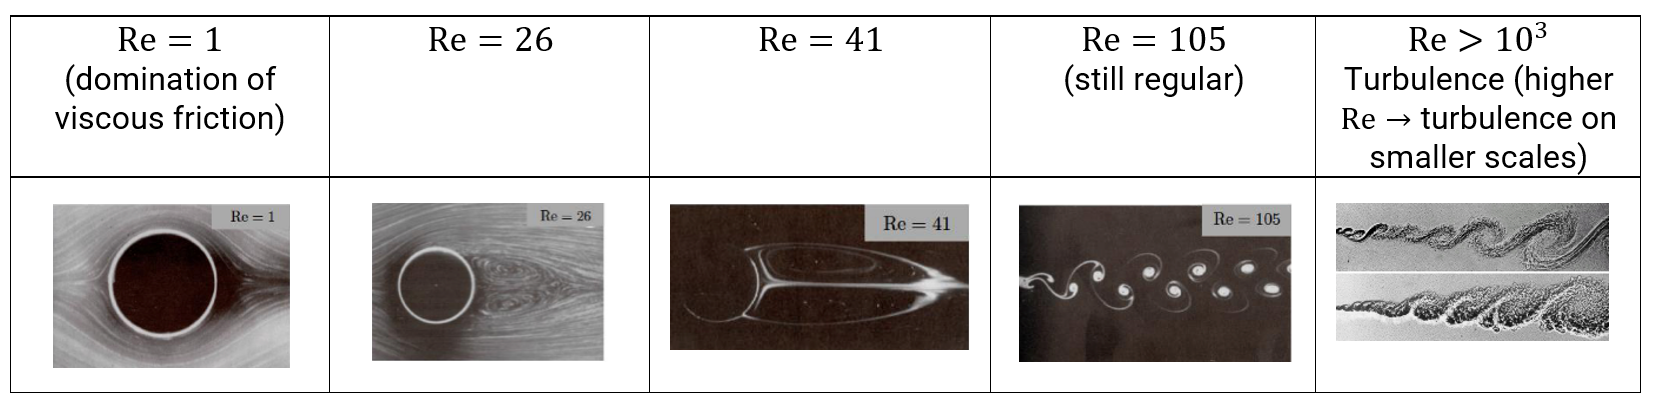
\includegraphics[width=0.95\textwidth]{figures/reynolds_numbers.png}
    \caption{Reynolds number}
    \label{fig:reynolds_number}
\end{figure}

\subsection{Shocks}
In hydrodynamical flows, shock waves can develop, where the fluid variables
\begin{itemize}
    \item density $\rho$
    \item velocity $\vec{v}$
    \item temperature $T$
    \item specific entropy $s$
\end{itemize}
jump by finite amounts. In the frame of the Euler equations these are
true mathematical discontinuities, while exhibiting a finite width in the Navier Stokes equations. A shock wave
\begin{itemize}
    \item propagates faster than the signal speed for compressible waves $c_s$
    \item causes an irreversible change to the fluid (increase in entropy)
\end{itemize}
A shock wave is a region of small thickness over which the properties of the flow change rapidly.

\subsubsection{Propagation of disturbances 1: Speed of sound}
\greenbox{\textbf{Microscopic Intuition:} Consider a higher density region in a fluid. Probabalisticly there is more momentum in the direction of lower density, so (by collisions) the higher density will spread out.
The characteristic speed of on which density information propagates is related to the jiggling of the particles, i.e. their themperature. 
This characteristic speed of sound is roughly derived in the following.}
\greenbox{Soundwaves are messengers, carrying density and pressure fluctuations. Imagine you're driving in fog towards a traffic jam - if you're so quick no messenger can quickly enough reach you, you will have a shock.}
Consider the Euler equation for momentum without internal forces
or friction in 1D in a steady state with constant flux $j = \rho v$, so
$0 = d(\rho v) \rightarrow \rho dv = -v d\rho$. We get

\begin{equation}
    \frac{dv}{dt} = -\frac{1}{\rho} \frac{dP}{dx} \quad \rightarrow \quad dP = -(\rho dv) \frac{dx}{dt} = (v d\rho) v \quad \rightarrow \quad v^2 \equiv c_s^2 = \frac{dP}{d\rho}
\end{equation}

(note is relative to the bulk motion, so in the local rest frame of the flow, more later).

Now we use that for an adiabatic process, $P \rho^{-\gamma} = \text{const.}$ (and $T\rho^{1-\gamma} = \text{const.}$) so taking the logarithm and differentiating with respect to $\rho$ yields

\begin{equation}
    \frac{dP}{d\rho} = \frac{\gamma p}{\rho}
\end{equation}

so using the ideal gas law

\begin{equation}
    P = n k_B T = \frac{\rho}{m_p \mu} k_B T \quad \text{with } \mu \text{ being a mean molecular weight}
\end{equation}

we get

\begin{equation}
    c_s^2 = \frac{\gamma k_B T}{m_p \mu}
\end{equation}

so based on $T\rho^{1-\gamma} = \text{const.}$ we can write

\begin{equation}
    c_s^2 \propto \rho^{\gamma - 1}
\end{equation}

\subsubsection{Characteristics of Perturbations}
\idea{Our aim is to find the characteristics, lines in the $(x,t)$ plane along which perturbations propagate.}
Let us start with the continuity equation in 1D

\begin{equation}
    \text{cont.: }\frac{1}{\rho} \left( \frac{\partial \rho}{\partial t} + v \frac{\partial \rho}{\partial x} \right) = 0
\end{equation}

With $c_s^2 = \frac{\partial P}{\partial \rho}$ we can write the Euler equation for momentum as

\begin{equation}
    \text{Euler: } \frac{\partial v}{\partial t} + v \frac{\partial v}{\partial x} = -\frac{1}{\rho} \frac{\partial P}{\partial x} = -\frac{c_s^2}{\rho} \frac{\partial \rho}{\partial x}
\end{equation}

Based on $c_s^2 \propto \rho^{\gamma - 1}$, we can replace $\partial \rho$ in those equations using
\begin{equation}
    \frac{d\rho}{\rho} = \frac{2}{\gamma - 1} \frac{dc_s}{c_s}
\end{equation}

With this replace $\partial \rho$ in the continuity and Euler equation. From adding
and subtracting the Euler and continuity equation, we get
\begin{equation}
    \begin{aligned}
        &\left[\partial_t+\left(v+c_{s}\right) \partial_x\right]\left(u+\frac{2}{\gamma-1} c_{s}\right)=0\\
        &\left[\partial_t+\left(v-c_{s}\right) \partial_x\right]\left(u-\frac{2}{\gamma-1} c_{s}\right)=0
    \end{aligned}
\end{equation}
Defining
\begin{equation}
    \begin{aligned}
        &\xi_{+} \equiv u+\frac{2}{\gamma-1} c_{s} \quad \rightarrow \quad \frac{d}{dt} \xi_{+}(x(t),t) = \left[ \partial_t + (\partial_t x) \partial_x \right] \xi_{+}(x(t),t) = 0 \text{ for } \partial_t x = v + c_s\\
        &\xi_{-} \equiv u-\frac{2}{\gamma-1} c_{s} \quad \rightarrow \quad \frac{d}{dt} \xi_{-}(x(t),t) = \left[ \partial_t + (\partial_t x) \partial_x \right] \xi_{-}(x(t),t) = 0 \text{ for } \partial_t x = v - c_s
    \end{aligned}
\end{equation}
where we applied the \textit{method of characteristics}.
\par
\begin{mdframed}[style = padded]
    From this we can see that (\textit{as expected}) in a fluid with bulk motion $v$, perturbations propagate along characteristics with velocity $v \pm c_s$.
\end{mdframed}

These characeteristic equations are the same no matter the aplitude of the perturbations.

\subsubsection{Formation of a shock}
\subsubsubsection{Formation as a pressure driven compressive disturbance}
\begin{figure}
    \centering
    \includesvg[width=0.9\textwidth]{figures/shock_formation.svg}
    \caption{Formation of a shock}
    \label{fig:shock_formation}
\end{figure}

Consider a fluid with base density $\rho_0$. For small perturbation in density, we can to first order
use
\begin{equation}
    c_s = \left( \frac{\partial P}{\partial \rho} \right)^{\frac{1}{2}} \simeq \left(\frac{\gamma p_0}{\rho_0}\right)^{\frac{1}{2}}
\end{equation}
But now consider a larger perturbation. Adiabatically the temperature scales with $T \propto \rho^{\gamma - 1}$, and as $c_s^2$ scales
linearly with the temperature, we have
\begin{equation}
    c_s^2 \propto T \propto \rho^{\gamma - 1} 
\end{equation}
Therefore, the “waves crest overtakes the valley” (figure \ref{fig:shock_formation}) but as the hydrodynamic equations don't allow for multivalued solutions, we get a shock
with discontinuities in $\rho$, $v$, $T$ and $s$. For an isothermal gas $c_s = \text{const.}$ but steepening can happen
nonetheless as of the non-linearity of the Euler / Navier-Stokes equations (?).

\subsubsubsection{Causes for shocks}
\begin{itemize}
    \item supersonic compressible disturbance
    \item supersonic collision of two streams of fluids
    \item non-linear interaction of subsonic compressible modes (nonliear wave interaction)
\end{itemize}

\subsubsection{Collisional and collisionless shocks | shock front}
The \enquote{discontinuous} change normally happens over a scale proportional to the \textit{effective} mean free path $\lambda_{eff}$.
\begin{itemize}
    \item Collisional shocks: Coulomb-collisions determine $\lambda_{eff}$
    \item Collisionless plasma like solar wind: $\lambda_{eff}$ is reduced by electromagnetic viscosities $\lambda_{eff} \ll \lambda_{coulomb}$
\end{itemize}

The shock front or transition layer is of the scale of $\lambda_{eff}$. Here, viscous effects are important - they dissipate kinetic energy, generating heat and entropy. Outside this layer viscous effects are small on scales $L \gg \lambda_{eff} \rightarrow \mat{\Pi} = \mat{0}$.

\note{This scale violates the assumptions under which the Navier-Stokes equations are derived from the Boltzmann equation. \enquote{It would be more than 50 years before computer simulation and laboratory experiments would show that physical shocks are measured to be twice the width predicted by theory, validating Becker's assertion that something beyond the Navier-Stokes description is needed.} \citep{Margolin2023}}

\subsubsection{Properties at fluid discontinuities}
External gravitational forces and conductive heat flux are way slower than the transition time
of fluid discontinuities and can thus be neglected.

We consider the propagating fluid discontinuity in its rest frame (i.e. upstream is ahead of the shock).

We distinguish \textcolor{blue1}{two types of fluid discontinuities}
\begin{itemize}
    \item shocks characterized by mass flux through their interface
    \item contact dicontinuities without such mass flux
\end{itemize}

\subsubsubsection{(Rankine-Hugoniot) Jump conditions I: Assumptions}
Relative to the shock, fluid moves from upstream to downstream and we would like to relate
upstream conditions $\rho_1,v_1,T_1$ to downstread conditions $\rho_2,v_2,T_2$ by \textit{jump conditions}, see figure \ref{fig:normal_shock}.

\begin{figure}[!htb]
    \centering
    \includesvg[width=0.9\textwidth]{figures/normal_shock3.svg}
    \caption{Normal shock}
    \label{fig:normal_shock}
\end{figure}

We assume
\begin{itemize}
    \item the velocity to be perpendicular to the surface of the discontinuity (we later generalize)
    \item a steady state $\partial_t = 0$
    \item a 1D situation $\vec{\nabla} \rightarrow \partial_x$
\end{itemize}

\subsubsubsection{(Rankine-Hugoniot) Jump conditions II: Jump condition from the continuity equation}
From the above assumption and the \textcolor{blue1}{continuity equation}, we following
\begin{equation}
    \begin{gathered}
        \frac{d}{dx} (\rho v) = 0 \rightarrow \rho v = \text{const.} \rightarrow \rho_1 v_1 = \rho_2 v_2 = j, \quad \text{mass flux } j \\
        v_1,v_2 \text{ measured in frame of the discontinuity} \\
        \text{notation for up-downstream-difference: } \boxed{[\rho v] = 0}
    \end{gathered}
\end{equation}
\textcolor{blue1}{The mass flux is constant across the discontinuity.}

\subsubsubsection{(Rankine-Hugoniot) Jump conditions III: Jump condition from the momentum equation}
One obtains (for the pre and post shock zones)
\begin{equation}
    \frac{d}{dx} (\rho v^2 + P) = 0 \quad \rightarrow \quad \boxed{[\rho v^2 + P] = 0}
\end{equation}
\note{We consider the difference in the pre- and post-shock-zones, where viscosity effects can be neglected ($\xi,\eta =0$)
and also $\frac{dv}{dx} = 0$. Note that as the transition zone is typically of a scale $\lambda_{mfp}$, we would
have to resort to kinetic theory (or plasma particle in cell-codes) there anyways.}

\subsubsubsection{(Rankine-Hugoniot) Jump conditions IV: Jump condition from the energy equation}
We obtain
\begin{equation}
    \begin{gathered}
        0 = \frac{d}{dx} \left( (\rho \mathcolor{blue1}{e} + P) v \right) = \frac{d}{dx} \left( \rho v \left( \mathcolor{blue1}{e_{th} + \frac{v^2}{2}} + \frac{P}{\rho} \right) \right) \\
        = \rho v \frac{d}{dx} \left( \left( e_{th} + \frac{v^2}{2} + \frac{P}{\rho} \right) \right) + \mathcolor{red1}{\frac{d(\rho v)}{dx}} \left( \left( e_{th} + \frac{v^2}{2} + \frac{P}{\rho} \right) \right) \underbrace{=}_{[\rho v] = 0} \rho v \frac{d}{dx} \left( \left( e_{th} + \frac{v^2}{2} + \frac{P}{\rho} \right) \right) \\
        \rightarrow \boxed{\left[ \frac{v^2}{2} + e_{th} + \frac{P}{\rho} \right] = 0}
    \end{gathered}
\end{equation}
Marked in the $\boxed{\text{boxes}}$ are the Rankine-Hugoniot Jump conditions.

We can plug in the closure $e_{th,i} = P_i / \left(\rho_i\cdot(\gamma_i -1) \right)$ into the energy jump condition
where theoretically $\gamma_i$ can be different in the pre- and post-shock zones, e.g. when molecules are
dissociated.

\subsubsubsection{Types of dicontinuities: contact discontinuity vs. shock}
The continuity of mass flux allows two scenarios
\begin{itemize}
    \item \textbf{tangential discontinuity}: $\mathcolor{blue1}{\rho_1v_1 = \rho_1 v_2 = 0}$ so as $\rho_1,\rho_2 \ne 0$ in general, $v_1=v_2=0$ so $[P] = 0$ as of $[\rho v^2 + P] = 0$. The pre- and post-shock zones move with the
    same velocity as the shock, there is no mass-flux through the shock. If the tangential velocities are also continuous ($[v_y] = [v_z] = 0$) (which we do not consider by our current assumptions), this is called a \textcolor{blue1}{contact dicontinuity}. The density may jump but as of $[P] = 0$, $T$ then has to do the \textit{opposite} jump. A contact discontinuity is a surface separating two fluids with different physical properties.
    \item \textbf{shock}: for $\mathcolor{blue1}{\rho_1v_1 = \rho_1 v_2 \ne 0}$ we have mass flux and thus a shock. Shock waves do propagate with respect to the fluid because of the mass flux in the normal.
\end{itemize}

\subsubsection{Characterizing the Shock strength - Mach number}

\note{In the shock's frameof reference, the unshocked material is moving at speed $v_1$ and the shocked material at speed $v_2$.}

The (pre-shock) Mach number is the ratio between the upstream (with respect to the shock) velocity to the upstream
sound speed, characterizing the strength of a shock ($\rho_1 v_1 \ne 0$) (in case of a jet causing the upstream
velocity, the jets velocity is used\footnote{If a jet is flying sufficiently fast, some of its energy goes into compressing the air in front. If the jet itself moves faster
than $c_s$, the information speed in the air, shock waves form as of those compressions (they cannot spread suffieciently fast
for there not to be a shock).})
\begin{equation}
    \mathcal{M}_1 \equiv \frac{v_1}{c_{s,1}} \underbrace{=}_{c_s^2 = \frac{\gamma P}{\rho}} \sqrt{\frac{\rho_1 v_1^2}{\gamma P_1}} \underbrace{=}_{P=\frac{\rho}{m}k_B T} \sqrt{\frac{mv_1^2}{\gamma k_B T_1}}
\end{equation}
we can analogously define a post-shock Mach number $\mathcal{M}_2$.

\begin{equation}
    \mathcal{M}_2 \equiv \frac{v_2}{c_{s,2}}
\end{equation}

Equivalently, the Mach number is
\begin{itemize}
    \item ratio of ram pressure $\rho v^2$ (pressure as of fluids bulk motion, not the thermal motion) to thermal pressure (for $\mathcal{M}_1$ in the pre-shock zone)
    \item and (as pressure is also an energy density) the kinetic thermal energy density
\end{itemize}

\note{Below $\mathcal{M} = 1$ there is no shock, the flow is subsonic.  A shock occurs, when supersonic flow (e.g. Solar Wind) encounters an obstacle forcing a change in velocity (e.g. the Earth's magnetosphere $\rightarrow$ bow shock).}

\subsubsubsection{Occurence of the Mach number in the continuity equation}
Rewriting $\partial_t \rho + \vec{\nabla} \left(\rho \vec{v} \right) = 0$ using $\frac{D}{Dt} = D_t = \partial_t + \vec{v} \cdot \vec{\nabla}$
to $-\frac{1}{\rho}\frac{D\rho}{Dt} = \vec{\nabla} \cdot \vec{v}$ and using the adiabatic $dp = c_s^2 d\rho$ we get
\begin{equation}
    -\frac{1}{\rho c_s^2} \frac{D\rho}{dt} = \vec{\nabla} \cdot \vec{v} \quad \xrightarrow{\text { dimensionless form }} \quad -\mathcal{M}^2 \frac{1}{\hat{\rho}} \frac{D\hat{\rho}}{D\hat{t}} = \vec{\hat{\nabla}} \cdot \vec{\hat{v}}
\end{equation}
So in the limit $\mathcal{M} \rightarrow 0$ we have incompressible flow.

\subsubsubsection{Rewriting the Rankine-Hugoniot jump conditions in terms of $\mathcal{M}_1$ - relating pre- and post-shock quantities}
One can rewrite the jump conditions in terms of the Mach number $\mathcal{M}_1$ (assume $\gamma_1 = \gamma_2 = \gamma$) (here
without proof)

\begin{equation}
    \begin{aligned}
    & \frac{\rho_2}{\rho_1}=\frac{v_1}{v_2}=\frac{(\gamma+1) \mathcal{M}_1^2}{(\gamma-1) \mathcal{M}_1^2+2} \stackrel{\gamma=1}{\longrightarrow} \mathcal{M}_1^2 \\
    & \frac{P_2}{P_1}=\frac{\rho_2 k_{\mathrm{B}} T_2}{\rho_1 k_{\mathrm{B}} T_1}=\frac{2 \gamma \mathcal{M}_1^2-(\gamma-1)}{\gamma+1} \stackrel{\gamma=1}{\longrightarrow} \mathcal{M}_1^2 \\
    & \frac{T_2}{T_1}=\frac{\left[(\gamma-1) \mathcal{M}_1^2+2\right]\left[2 \gamma \mathcal{M}_1^2-(\gamma-1)\right]}{(\gamma+1)^2 \mathcal{M}_1^2} \stackrel{\gamma=1}{\longrightarrow} 1
    \end{aligned}
\end{equation}

from which we for a strong shock ($\mathcal{M}_1 \gg 1$)\footnote{In a strong shock $v_1^2 \gg c_1^2$, so the thermal pressure of the unshocked gas is negligible to its ram pressure.} can find (use $\gamma = 5 / 3$ for an ideal non-relativistic gas)

\begin{equation}
    \begin{aligned}
    \frac{\rho_2}{\rho_1} & =\frac{v_1}{v_2} \approx \frac{\gamma+1}{\gamma-1}=4, \\
    P_2 & \approx \frac{2 \gamma}{\gamma+1} \mathcal{M}_1^2 P_1=\frac{2}{\gamma+1} \rho_1 v_1^2=\frac{3}{4} \rho_1 v_1^2, \\
    k_{\mathrm{B}} T_2 & \approx \frac{2 \gamma(\gamma-1)}{(\gamma+1)^2} k_{\mathrm{B}} T_1 \mathcal{M}_1^2=\frac{2(\gamma-1)}{(\gamma+1)^2} m v_1^2=\frac{3}{16} m v_1^2,
    \end{aligned}
\end{equation}

In the shock frame, the post-shock medium is slower, denser, has higher-pressure and is warmer, see figure \ref{fig:shock_mach}.

\begin{figure}[!htb]
    \centering
    \includesvg[width=0.9\textwidth]{figures/shock_mach.svg}
    \caption{Relation of pre- and post-shock quantities (shock $\rightleftarrows$ $\mathcal{M}_1 = \frac{v_1}{c_1}> 1$). $v_1$ is the velocity of the upstream (pre-shock) fluid with respect to the shock.}
    \label{fig:shock_mach}
\end{figure}

\subsubsubsection{Conversion of kinetic to thermal energy in the shock}
Based on the above relations for $\mathcal{M}_1 \gg 1, \gamma = 5/3$ we can write
\begin{equation}
    \begin{gathered}
        \text{post-shock specific kinetic energy: } \frac{1}{2} v_2^2 \approx \frac{1}{16} \frac{1}{2} v_1^2 \\
        \text{post-shock specific thermal energy: } \frac{3}{2} \frac{k_B T_2}{m} \approx \frac{9}{32} v_1^2 = \frac{9}{16} \frac{1}{2} v_1^2
    \end{gathered}
\end{equation}
We find that in the shock frame, roughly half of the pre-shock kinetic energy ($\frac{9}{16}$) is converted to thermal energy.

\subsubsubsection{Conservation of energy in the shock}
In the pre-shock flow (for a strong shock) we can neglect the thermal energy, so $e_1 = \frac{v_1^2}{2}$ (specific energy per particle).

In
\begin{equation}
    \frac{1}{2} v_2^2 + \frac{3}{2} \frac{k_B T_2}{m} \approx \frac{10}{16} \frac{v_1^2}{2}
\end{equation}
(in the shock rest frame) one is missing the $p dV$ work, which is done by the shock to compress the post-shock gas
and amounts to $k_B T_2 \approx \frac{6}{16} \frac{1}{2} v_1^2$.
\note{The sum of enthalpy (thermal energy + $p dV$ work) and kinetic energy is conserved in adiabatic flow (even when
non-adiabatic processes like shocks occur between the two sections). Enthalpy plays the same role in a flowing
system that internal energy takes in a non-flowing one, taking care of the energy associated with
flow work in / out of the control volume.}

\note{There are also radiative shocks, where in the transition through the shock energy is radiated away.}

\note{In the rest frame of the post-shock gas there is no $P dV$ term.}

\subsubsubsection{Connection between pre- and post-shock Mach number}
We can write the post-shock Mach number as
\begin{equation}
    \mathcal{M}_2 = \frac{v_2}{c_2} = \frac{v_1}{c_1} \frac{v_2}{v_1} \frac{c_1}{c_2} \underbrace{=}_{c^2\propto T} \mathcal{M}_1 \frac{v_2}{v_1} \left(\frac{T_1}{T_2}\right)^{\frac{1}{2}}
\end{equation}
Plugging in the jump condition for $T_2 / T_1$, in the strong shock limit we get
\begin{equation}
    \mathcal{M}_2 = \left( \frac{\gamma - 1}{2\gamma} \right) ^ {\frac{1}{2}} \underbrace{\approx}_{\gamma = 5/3} 0.45
\end{equation}
\greenbox{\textbf{Summary:} Supersonic gas is slowed down (to subsonic), compressed (density, pressure and temperature increase) by a shock.}

\subsubsubsection{Shock adiabatic curve\skipthis}
\note{In shocks, the post-shock entropy is increased with respect to the pre-shock entropy - the shock shifts the gas to a higher adiabatic curve.}
The shock is a non-adiabatic process ($\delta Q \ne 0 \rightarrow dS = \frac{\delta Q}{T} \ne 0$).
Based on the first law of thermodynamics $\delta Q = dE + P dV$, the ideal gas law and $dE = \nu c_V dT$ (number of mols $\nu$), we can
one can find for an ideal polytropic gas that $s = c_V \ln{\left( \frac{p}{\rho^\gamma} \right)}$, so here

\begin{equation}
    s_2 - s_1 = c_V \ln{\left( \frac{p_2}{p_1} \left( \frac{\rho_1}{\rho_2} \right)^\gamma \right)} = c_V \ln{\left( \frac{K_2}{K_1} \right)}
\end{equation}

The shock shifts the gas to a higher adiabatic curce $K=P\rho^{-\gamma}$. Note that one finds using the jump conditions, that $s_2 - s_1 > 0$ only
for $\mathcal{M}_1 > 1$, so there is only a shock for $\mathcal{M}_1 > 1$.

Based on $j=\rho_1 v_1 = \rho_2 v_2$ and $[\rho v^2 + P] = 0$ the slope of the shock adiabatic curve in a PV-diagram is
\begin{equation}
    \frac{j^2}{m} = \frac{P_2 - P_1}{V_1 - V_2}
\end{equation}

$P = \text{const.} \times \rho^\gamma$ on either side of the shock (where we assume equilibrium), but with different constants.

\note{The jump conditions are \textit{reversible} - if we interchange post- and pre-shock flow conditions, so $v_1 < v_2$, then density, pressure and temperature would decrease across the shock and so the entropy, excluding a shock with expansion.}

\subsubsubsection{Oblique shocks}
The fluid might not impact the shock perpendicular to the shock front, but at an oblique angle.
\textbf{Result:} The shock deflects the flow away from the shocks normal direction (towards the shock's surface), the final velocity may remain supersonic. 
Only the velocity component normal to the shock front changes, $V_t$ is continuous across the shock (see figure \ref{fig:oblique_shock}).

\begin{figure}[!htb]
    \centering
    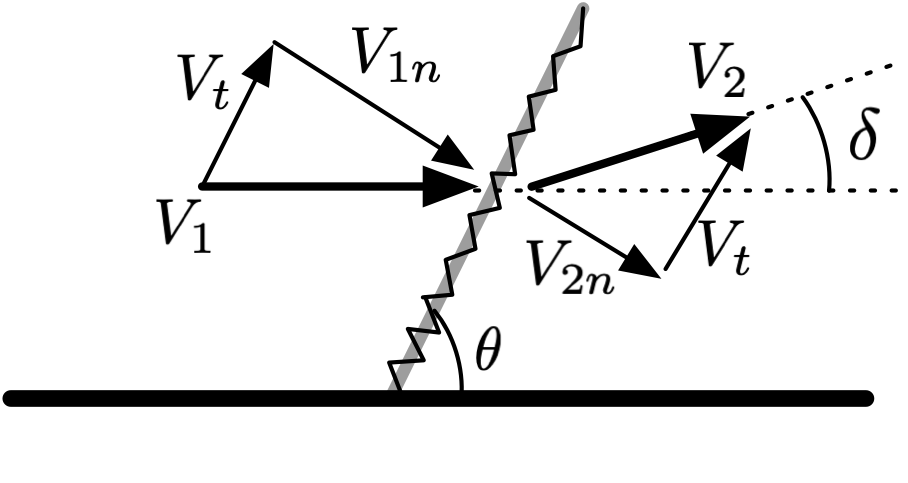
\includegraphics[width=0.7\textwidth]{figures/oblique-shock.png}
    \caption{Oblique shock}
    \label{fig:oblique_shock}
\end{figure}

\textbf{Derivation - oblique jump conditions:} Let $\vec{n}$ (here $=\vec{\hat{e}}_x$) be the shock normal, so $v_\parallel = \vec{v} \cdot \vec{n}$ is the component of the fluid velocity $v$ parallel and $v_\perp$ the one perpendicular to $\vec{n}$.
The Navier-Stokes equation describes conservation of momentum in form of a continuity equation and as such contains a momentum current.
This current across the shock, $\rho \vec{v} (\vec{v} \cdot \vec{n})$, is continuous across the shock, yielding
\begin{equation}
    \begin{aligned}
        [\rho v_x^2 + P] &= 0 \\
        [\rho v_x v_y] &= 0 \\
        [\rho v_x v_z] &= 0
    \end{aligned}
\end{equation}
As we are dealing with a shock with momentum flux $[\rho v_x] \ne 0$, we get
\begin{equation}
    [v_y] = 0, \quad [v_z] = 0
\end{equation}
so as stated, the tangential velocities are continuous across the shock, $v_{1,\perp} = v_{2,\perp} = v_\perp$ and
for $v_{2,\parallel}$ we have $v_{2,\parallel} = v_{1,\parallel} \frac{\rho_1}{\rho_2}$ ($\rho_2 > \rho_1$).
So if the component parallel to the shock normal gets smaller and the one perpendicular remains the same, we
are deflected away from the shock normal.

\subsection{Fluid instabilities}
Instabilities are the rapid growth of small perturbations, tapping into a source of free energy.

\subsubsection{Stability of a shear flow}
We consider two flows counterpropagating side by side (see figure \ref{fig:shear_flow}). Using perturbation theory, the stability
of the flow can be analyzed - if the dispersion relation for a perturbation yields a positive imaginary part (not just yeal oscillation)
such modes grow exponentially - the flow is unstable.

\begin{figure}[!htb]
    \centering
    \includesvg[width=0.9\textwidth]{figures/shear_flow2.svg}
    \caption{Shear flow}
    \label{fig:shear_flow}
\end{figure}

\subsubsection{Rayleigh-Taylor instability}
Here we consider a fluid at rest, i. e. $v_1=v_2=0$. If the denser fluid lies on top, there are unstable solution - Rayleigh-Taylor instability.
The instability is driven by the buoyancy of the lighter fluid or rather the release of potential energy with respect to the external force $\vec{g}$ (see figure \ref{fig:rayleigh_taylor}).
If the denser fluid is on the bottom, the interface is stable and will only oscillate if perturbed. There is also the Rayleigh-Taylor instability in plasmas.

\begin{figure}[!htb]
    \centering
    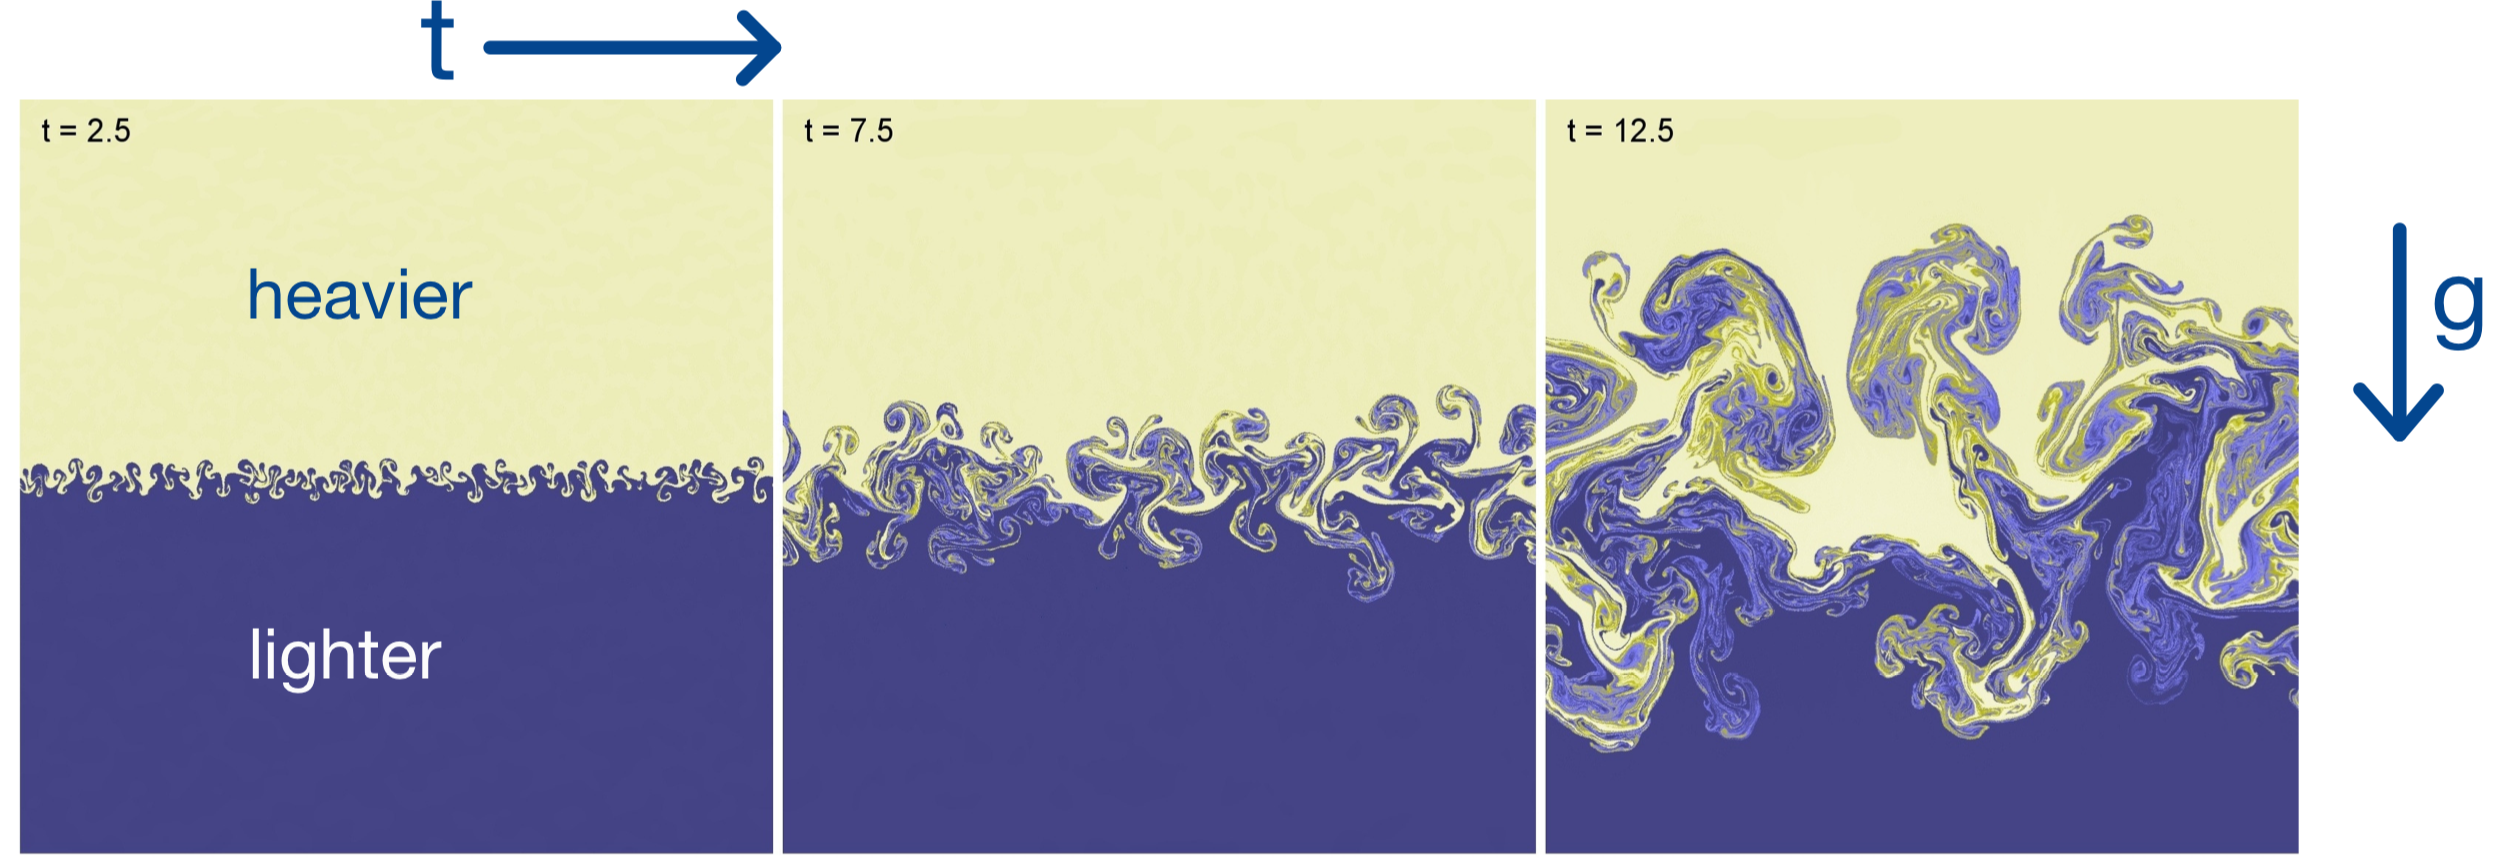
\includegraphics[width=0.9\textwidth]{figures/rayleigh_taylor.png}
    \caption{Rayleigh-Taylor instability}
    \label{fig:rayleigh_taylor}
\end{figure}

\subsubsection{Kelvin-Helmholtz instability}
Consider the case without the gravitational field $\vec{g} = 0$. In an ideal gas, small wave like perturbances will grow into large waves (with largest growth for large $k$, so small wavelengths) - Kelvin-Helmholtz-Billows, which subsequently roll up to vortex-like structures.
Sharp velocity gradients are unstable - we can create turbulence.
Some modes can be stabilized against the instability if we have the gravitational field, the heavy part is on the bottom (otherwise Rayleigh-Taylor instability) and
the velocity difference $(v_2 - v_1)^2$ is sufficiently small.

\subsubsection{Further instabilities}
\begin{itemize}
    \item \textbf{Richtmyer-Meshkov instability}: at suddenly accelerated interfaces
    \item \textbf{Jeans-instability}: in self-gravitating fluids, where denser regions can grow and collapse under their own attraction
    \item \textbf{Thermal instbaility}: $\dots$
\end{itemize}


\subsection{Turbulence}
\enquote{Big whirls have little whirls that feed on their velocity, and little whirls have lesser whirls and so on to viscosity.} - Lewis Fry Richardson

Both laminar and turbulent flow are solutions to the 
deterministic Navier-Stokes equations, however turbulent flow
is chaotic, laminar not (see table \ref{tab:turbulence} and figure \ref{fig:turbulence}).

\begin{table}[!htb]
    \centering
    \begin{tabular}{|p{0.45\textwidth}|p{0.45\textwidth}|}
        \hline
        \textbf{Laminar flow} & \textbf{Turbulent flow} \\
        \hline
        Fluid flows in parallel layers with no disruption between those layers & Unsteady, chaotic flow with varying velocity and pressure in position and time \\
        \hline
        similar conditions $\rightarrow$ similar solutions & infinitesimal difference in conditions $\rightarrow$ vastly different solutions (deterministic chaos\footnote{When the present determines the future, but the approximate present does not approximately determine the future.}) \\
        \hline
    \end{tabular}
    \caption{Laminar vs. turbulent flow}
    \label{tab:turbulence}
\end{table}

\begin{figure}[!htb]
    \centering
    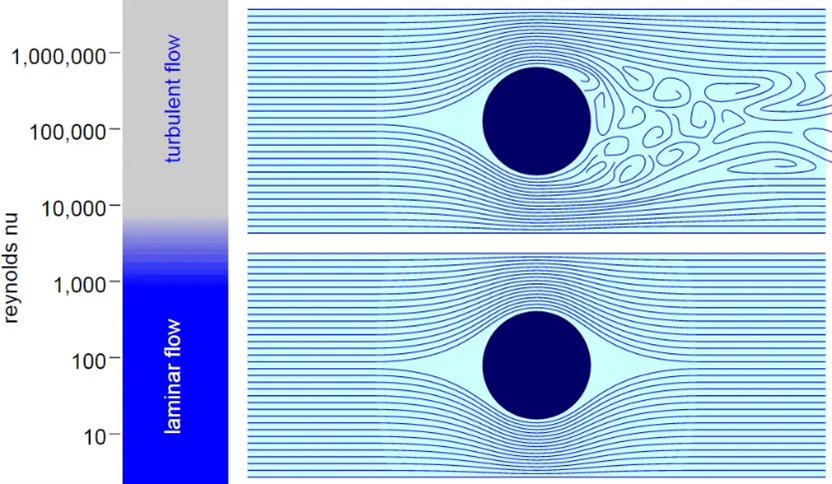
\includegraphics[width=0.4\textwidth]{figures/turbulence.png}
    \caption{Laminar vs. turbulent flow}
    \label{fig:turbulence}
\end{figure}

\subsubsection{Subsonic (incompressible) turbulence, low Mach numbers | rotational modes}
For subsonic turbulence, the information speed is far higher than the transport speed limiting
the naturally occuring compressions (no shocks), so we can assume the fluid to be incompressible, $\vec{\nabla} \cdot \vec{v} = 0$.

In Fourier space the nabla operator becomes $\vec{\nabla} \rightarrow \vec{k}$, so $\vec{k} \cdot \vec{v} = 0$, so there
are no longitudinal disturbances (aka soundwaves) but only solenoidal, i.e. source free motion, so shear flow and rotational turbulence
(swirling eddies as for instance produces by the Kelvin-Helmholtz instability).

$\vec{\nabla} \cdot \vec{v} = 0$ also implies subsonic flow as supersonic velocities would cause shocks coming with compression of the post-shock fluid.

\textcolor{blue1}{Incompressible turbulence is described by Kolmogorov's theory of incompressible turbulence}.

Incompressible flow is governed by the Navier-Stokes equation for an incompressible fluid, so

\begin{equation}
    \partial_t \vec{v} + \overbrace{(\vec{v} \cdot \vec{\nabla}) \vec{v}}^{\text{advective transport}} = \vec{g} \underbrace{- \frac{1}{\rho} \vec{\nabla} P}_{\text{pressure force}} + \overbrace{\nu \nabla^2 \vec{v}}^{\text{viscous dissipation}}
\end{equation}

\subsubsection{How to quantify turbulence? - Reynolds number}
Let us come back to the Reynolds number characterizing the ratio of the advective to the friction term in the Navier-Stokes equation

\begin{equation}
    \begin{gathered}
        Re = \frac{\text{advective term}}{\text{frictional term}} = \frac{|(\vec{v}\cdot \vec{\nabla})\vec{v}|}{\nu \vec{\nabla}^2 \vec{v}} = \frac{V_0 L_0}{\nu} \\
        \text{with } V_0 = \text{characteristic velocity}, \quad L_0 = \text{characteristic length scale}, \\ \nu = \text{kinematic viscosity} = \frac{\eta}{\rho} \sim \lambda_{mfp} v_{th} \\
        \text{with } \lambda_{mfp} = \text{mean free path}, \quad v_{th} = \text{thermal velocity}
    \end{gathered}
\end{equation}

Although counterintuitive, the viscosity increases with larger mean free path, intuitively as shear stress information is transported
over larger distances.

In this view a high Reynolds number means that turbulence is generated faster by the chaotic advective term than is descroyed via dissipation.

\begin{mdframed}[style=padded]
    For approximately $Re > 3.5 \cdot 10^3$ turbulence is expected, the interstellar medium has $Re \sim 10^{8}$. Oceans (viscosity of water $\sim 10^{-6} \m^2 \s^{-1}$) and atmosphere are always turbulent, except for boundary layers (with small characteristic length scale).
\end{mdframed}

\subsubsubsection{Reynolds number as the ratio between advection and dissipation timescale}
Most simply by dimensional analysis, one can yield ($\nu$ in units of $\frac{m^2}{s}$, a diffusion coefficient)
\begin{equation}
    t_{adv} = \frac{L_0}{V_0}, \quad t_{dis} = \frac{L_0^2}{\nu} \quad \rightarrow \quad Re = \frac{t_{dis}}{t_{adv}} = \frac{L_0 V_0}{\nu} \sim \frac{L_0 V_0}{\lambda_{mfp} v_{th}}
\end{equation}
where a high Reynolds number means that advection is faster than dissipation, thus dissipation cannot stabilize
the growth of turbulence sufficiently and we have turbulent flow. In the equation we can also see that the Reynolds number
is the product of the macroscopic-to-microscopic length and velocity scales.

\subsubsection{Supersonic turbulence, shocks $\mathcal{M} \gg 1$ | rotational and compressive modes}
Depending on the dimensionality, we have
\begin{itemize}
    \item 1D: 1 compressive mode
    \item 2D: 1 compressive mode, 1 solenoidal mode
    \item 3D: 1 compressive mode, 2 solenoidal modes
\end{itemize}

\subsubsection{Schematic concept of turbulence}
In 3D
\begin{itemize}
    \item \textbf{injection range} energy is injected on macroscopic scales, typical scale $L$, velocity $v$
    \item \textbf{inertial range} large eddies break up into smaller eddies and energy is transferred to smaller scales, vorticity ($\vec{\zeta} = \vec{\nabla}\times \vec{v}$) is conserved and no energy is dissipated
    \item \textbf{dissipation range} at the microscopic viscous scale ($\lambda_{visc}$, roughly the mean free path $\lambda_{mfp}$) energy is dissipated into viscous heat
\end{itemize}
In 2D the energy flow is reverted from small to large (inverse cascade).

\subsubsection{Kolmogorov scales of turbulence}
In the following consider
\begin{equation}
    \begin{gathered}
        \text{largest eddy scale: } L_S, \quad \text{dissipation scale: } L_k \\
        \text{rate of energy dissipation on small scales, energy flow in the inertial range: } \epsilon \\
        \text{some eddy size: } \lambda, \quad \text{velocity on that scale: } v_\lambda \\
        \text{fluid viscosity: } \nu \text{ in } \frac{m^2}{s} \\
    \end{gathered}
\end{equation}
\subsubsubsection{Dissipation scale - smallest scale to be resolved in a simulation}
Assume high Reynolds number and start at the small scale. At the small scale, turbulent motions are statistically
isotropic (different from the large scales $L_S$) and Kolmogorov postulates the statistics to be universally
determined by $\nu$ and $\epsilon$ (in $\m^2 / \s^3$). From dimensional analysis (physical units), one can then
get
\begin{equation}
    L_K \sim \left( \frac{\nu^3}{\epsilon} \right)^{\frac{1}{4}}
\end{equation}
\note{This is the smallest scale to be resolved in a classical simulation, for an airplane with chord length $2\m$ this is $\mathcal{O}(10^{-6})\m$ - quite a problem for simulations.}

\subsubsection{Scaling of the eddy velocity and vorticity in the inertial range}
Energy flow $\epsilon$ must be constant in the inertial range (otherwise accumulation).
We approximate the energy flow by the kinetic energy of an eddy divided by its characeteristic time scale
\begin{equation}
    \epsilon \approx \left( \frac{v_\lambda^2}{2} \right) \left(\frac{v_\lambda}{\lambda} \right) \approx \frac{v_\lambda^3}{\lambda} \underbrace{\approx}_{\epsilon = \text{const.}} \frac{v_{L_S}^3}{L_S}
\end{equation}
therefore, we get
\begin{equation}
    v_\lambda \approx v_{L_S} \left( \frac{\lambda}{L_S} \right)^{\frac{1}{3}}
\end{equation}
\note{The largest eddies have highest velocities.}
But as the size scales down quicker than the velocity, smallest eddies have the highest vorticity
\begin{equation}
    |\vec{\zeta}_\lambda| \approx \frac{v_\lambda}{\lambda} \approx \frac{v_{L_S}}{(\lambda^2 L_S)^{\frac{1}{3}}}
\end{equation}
\note{As the vorticity increases with decreasing scale but overall vorticity is approximately constant ($\sim$ conservation of angular momentum) on smaller scales less volume is filled with turbulent eddied.}

\subsubsection{Power spectrum of Kolmogorov turbulence}
The dissipation is reflected by the energy spectrum of Kolmogorov turbulence, see figure \ref{fig:kolmogorov_spectrum}.

\begin{figure}[!htb]
    \centering
    \includesvg[width=0.9\textwidth]{figures/kol_power.svg}
    \caption{Kolmogorov energy spectrum}
    \label{fig:kolmogorov_spectrum}
\end{figure}

The constant energy transfer through the cascade is described by
\begin{equation}
    \begin{gathered}
        \text{incompressible fluid, subsonic: } E(k) \propto k^{-\frac{5}{3}} \\
        \text{compressible, shock-dominated: } E(k) \propto k^{-2}
    \end{gathered}
\end{equation}

\note{Including the the dissipation range, based on Kolmogorovs assumption that the statistics for small scale motion are universal, one might make the ansatz $E(k) = C \epsilon^{\frac{2}{3}} k^{-\frac{5}{3}} f_\eta(k\eta)$ with $f_\eta(x) = 1$ for $x \ll 1$ and $f_\eta(x) \rightarrow 0$ for $x \rightarrow \infty$.}

\subsubsubsection{Derivation of the energy spectrum of Kolmogorov turbulence}
We are interested in the energy spectrum $E(k)$ such that the energy between
$k$-vectors ($k = 2\pi \slash \lambda$, length-scale $\lambda$) $k_1$ and $k_2$ is
\begin{equation}
    \Delta E = \int_{k_1}^{k_2} E(k) \, dk
\end{equation}
\begin{itemize}
    \item epxress the energy spectrum via the velocity power spectrum $P_v(k)$, 
    \begin{equation}
        E(k) \, dk = P_v(k) k^2 \, dk
    \end{equation}
    \item use that the power spectrum is the Fourier transform of the correlation function (so have the same scaling $P_v(k) \propto \lambda^3 \xi_v$), so here
    calculate
    \begin{equation}
        \xi_v(y) = \langle \vec{v}(\vec{x}) \cdot \vec{v}(\vec{x}+\vec{y}) \rangle \propto v_\lambda^2 \propto (\epsilon \lambda)^{\frac{2}{3}}
    \end{equation}
    (not dependent on the direction of $\vec{y}$ as turbulence is isotropic) with which we get the $k^{-\frac{5}{3}}$ scaling of the energy spectrum $E(k)$.
\end{itemize}

\pagebreak